\chapter{Grundlagen}
\label{chap:Grundlagen}
Im folgenden Kapitel werden die Grundlagen der Arbeit, insbesondere im Hinblick auf die gewählten Ansätze beschrieben. Begonnen wird mit den theoretischen Grundlagen, den Verwandten Arbeiten, gefolgt von einer Beschreibung der bestehenden Systeme, auf welche mit einem Abschnitt über die Daten und ihrer Vorverarbeitung abgeschlossen wird.

	\section{Autoencoder}
	\label{sec:ConvolutionalAutoencoder}		
	Autoencoder \cite{D.E.Rumelhart.1987} sind Werkzeuge, welche insbesondere zum Finden von Repräsentationen eingesetzt werden. Dabei komprimieren sie die Eingabe in einen niedrigdimensionaleren Raum und rekonstruieren aus diesem Code die Eingabe. Konkret besteht ein Autoencoder aus drei Teilen, dem Encoder, dem Codelayer und dem Decoder. In Abbildung \ref{img:SchemaCAE} ist das Schema eines Autoencoders abgebildet.
			\begin{figure}[h]
				\centering
				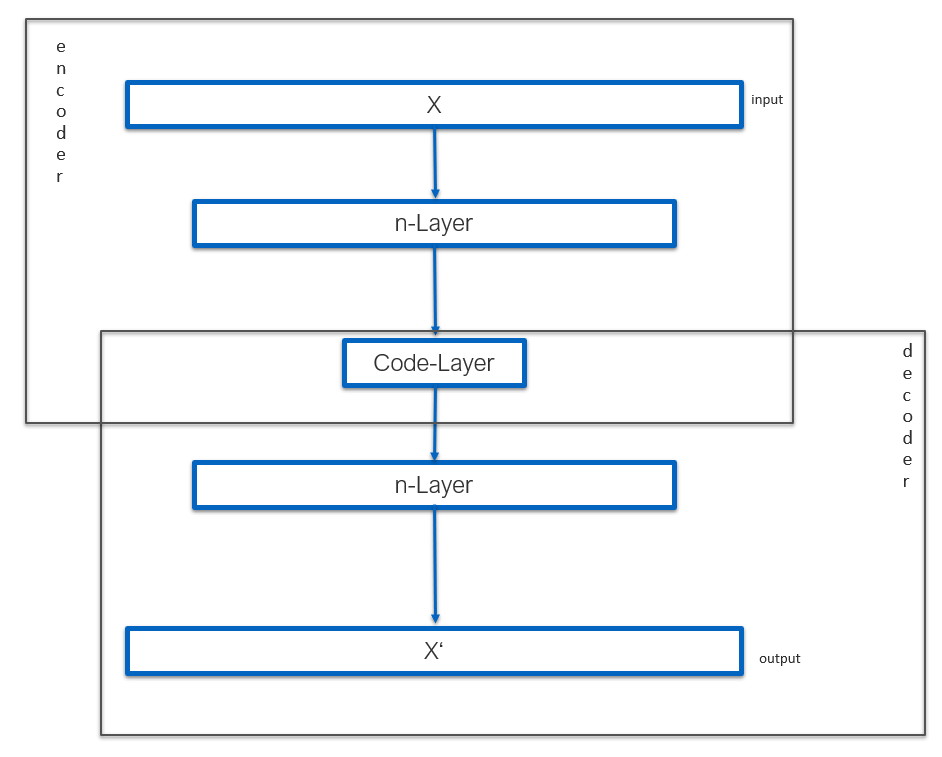
\includegraphics[width=0.7\textwidth, center]{bilder/Schema_Autoencoders/Schema_CAE2.png}
				\caption[Schema Autoencoder]{Schema Autoencoder}
				\label{img:SchemaCAE}
			\end{figure} 
	In der einfachsten Form besteht ein Autoencoder aus einer Eingabeschicht, einer versteckten Schicht und eine Ausgabeschicht. Sie können aber auch mit mehreren Schichten, also mit 'tiefen Architekturen' genutzt werden. \cite{Hinton.2006}
	Der Encoder lässt sich auch vereinfacht als die Funktion $F(x)=c$ und der Decoder als die Funktion $ F(c)=x'$ darstellen, wobei $x\stackrel{!}{=}x'$ sein soll. 
	Autoencoder gibt es in vielen verschiedenen Ausführungen. Dabei sind die meisten Typen von Autoencoder unvollständige Autoencoder. Die verborgene Schicht, das Codelayer enthält weniger Informationen als die Eingabe. Hierdurch wird die Dimensionsreduzierung erzwungen. Andere Aufgaben können Entrauschung mittels Denoising autoencoder \cite{Vincent.2008} oder Generierung neuer Datenpunkte mittels Varrational Autoencoder \cite{Kingma.2019} sein. Contractive Autoencoder \cite{Rifai.2011} nutzen einen Regularisierer in der Zielfunktion, um das Modell zu zwingen eine Funktion zu lernen, die flexibler auf Variationen der Eingabewerte reagiert.   	

	Für die Arbeit ist der \acl{cae} \cite{Masci.2011} kurz \ac{cae} interessant. Er ist ist ein Stacked Autoencoder, welcher Faltungsschichten (Convolutional Layer) \cite{LeCun.1999} integriert.  \todo{Convolutional Layer hier als Stand der Technik? CNN kommen von x haben sich durchgeserzt in 1,2,3,4,5}

	\paragraph{Schichtenweise Vortrainieren} Im schichtenweise Vortrainieren \cite{Bengio.2007}  werden einzelne Schichten eines neuronalen Netzwerkes vor dem eigentlichen Training trainiert, um die Leistung des gesamten Models zu erhöhen. Bei (symmetrischen) Autoencodern werden dabei die zueinander symmetrischen Schichten des Encoders und Decoders miteinander trainiert. Die Zielgröße ist dabei die Rekonstruktion der Eingabedaten.    

	\section{ Transferlernen}
	\label{sec:Transferlernen}
	Im traditionellen maschinellem Lernen wird pro Aufgabe und Datenset ein isoliertes Modell erstellt. Das Transferlernen hat das Ziel Wissen zu teilen. Die Isolation der Modelle soll aufgehoben werden. Dabei erfolgt eine Aufteilung in Quell- und Zieldomäne.
	
		\subsection{Tiefes Transferlernen}
		Geprägt durch die Entwicklung hin zu tiefen neuronalen Netzwerken wurden Methoden zum Tiefen Transferlernen (deep transfer learning) vorgeschlagen. \cite{Tirumala.2018} ordnet diese in vier Kategorien ein. Für eine Einordnung von klassischen Methoden des Transferlernens eignet sich die Erhebung \cite{FuzhenZhuang.2019}.
		     
		\paragraph{Instanzbasiert} Instanz-basierte Ansätze ergänzen, mittels geeigneter Strategie, Gewichte in der Zieldomäne mit Gewichten aus der Quelldomäne.
		\paragraph{Abbildungbasiert} Abbildungs-basierte Ansätze bilden Instanzen aus der Quell- und Zieldomäne in einen neuen Datenraum ab. In dem neuen Datenraum sind die Instanzen aus den zwei Bereichen ähnlich und können für ein gemeinsames Training eines tiefen neuronales Netzwerk genutzt werden. 
		\paragraph{Netzwerkbasiert} Der netzwerkbasierte Ansatz verwendet einen Teil des in der Quelldomäne trainierten Netzwerkes in der Zieldomäne wieder. Es werden dabei sowohl die Netzstruktur als auch die Verbindungsparameter übernommen. Die Netzwerke werden dabei in zwei Teile unterteilt. Der erste Teil ist die sprachunabhängige Merkmalstransformation, der zweite Teil ist der sprachabhängige Klassifikator. Dabei kann die sprachunabhängige Merkmalstransformation in der Zieldomäne wiederverwendet werden. \todo{related work? hier / eigenes kapitel}  
		\paragraph{Gegnerischbasiert} Gegenerischbasiertes tiefes Transferlernen ist von dem Ansatz erzeugende gegnerische Netzwerke (Generative Adversarial Networks) \cite{IanJ.Goodfellow.2014} inspiriert. Es werden übertragbare Repräsentationen gesucht, die sowohl auf die Quell- als auch auf die Zieldomäne anwendbar sind.

		\subsection{Halbüberwachtes Lernen}
		Halbüberwachtes Lernen ist eine Methode, die sich zwischen unüberwachtem und überwachtem Lernen einordnen lässt. Methoden des unüberwachten Lernens arbeiten komplett ohne annotierte Daten, während überwachtes Lernen mit vollständig annotierten Daten arbeitet. Das halbüberwachte Lernen arbeitet mit teilweise annotierten Daten. Die Anzahl der nicht annotierten Daten übersteigt, in der Regel, die Menge der annotierten Daten. Diese Technik reduziert Annotationskosten durch den Einsatz weniger Daten mit Annotationen. Zu beachten ist dabei, dass sowohl die Beschrifteten als auch nicht beschriftete Daten aus der gleichen Verteilung entnommen werden. 
		Im Gegensatz dazu sind bei dem Transferlernen die Datenverteilungen der Quell- und Zieldomäne oft unterschiedlich.
		\cite{Chapelle.2010} 
				
		\subsection{Multi-Task-Lernen}
		Werden mehrere Aufgaben parallel gelernt spricht man von dem \acl{mtl} kurz \ac{mtl}. Ziel ist es, Wissen durch gleichzeitiges Lernen einiger verwandter Aufgaben weiterzugeben. Es wird davon ausgegangen, dass das Lernen einer Aufgabe das Lernen der anderen Aufgaben verbessert. Im Allgemeinen wird dies durch das Lernen aller Aufgaben gemeinsam erreicht, wobei die korrelierten Informationen zwischen den einzelnen Aufgaben genutzt werden. Die Aufgaben erzeugen dabei eine niedrigdimensionale Repräsentation, welche dann durch das parallele Lernen besser generalisiert. In manchen Fällen hat sich zudem herausgestellt, dass Multi-Task-Lernen zum Lernen von nicht verwandten Aufgaben vorteilhaft ist.
		Basierend auf den Ein- und Ausgängen wird \ac{mtl} in drei Fälle unterteilt. 
 		
 		\paragraph{Single-Input Multi-Output} SIMO wird verwendet, um aus einer Eingabe Vorhersagen von verschiedenen Arten von Ausgabezielen zu treffen. Diese Art des \ac{mtl} wird auch Mehrklassen-Lernen (multi-class learning) genannt.
		
		\paragraph{Multi-Input Single-Output} MISO bedeutet es werden mehrere Eingaben zum Vorhersagen eines Ausgabezieles genutzt.
	
		\paragraph{Multi-Input Multi-Output} MIMO bedeutet es werden mehrere Eingaben zum Vorhersagen von verschiedenen Arten von Ausgabezielen genutzt.
		
		\begin{figure}[h]
			\centering
			\begin{subfigure}[c]{0.6\textwidth}			
				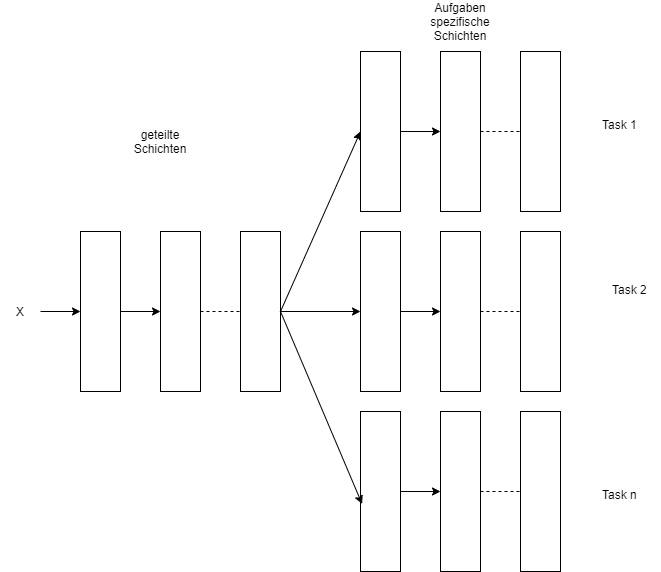
\includegraphics[width=1\textwidth, center]{bilder/Grundlagen/MTL/MTL_SIMO.png}
				\caption[MTL-SIMO]{Single-Input Multi-Output}
				\label{img:MTL_SIMO}	
			\end{subfigure}
			\begin{subfigure}[c]{0.49\textwidth}			
				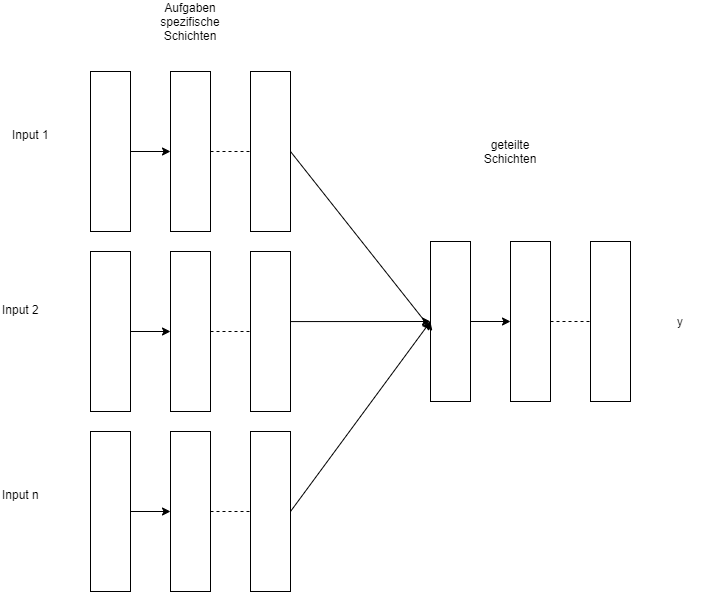
\includegraphics[width=1\textwidth, center]{bilder/Grundlagen/MTL/MTL_MISO.png}
				\caption[MTL-MISO]{Multi-Input Single-Output}
				\label{img:MTL_MISO}	
			\end{subfigure}
			\begin{subfigure}[c]{0.49\textwidth}			
				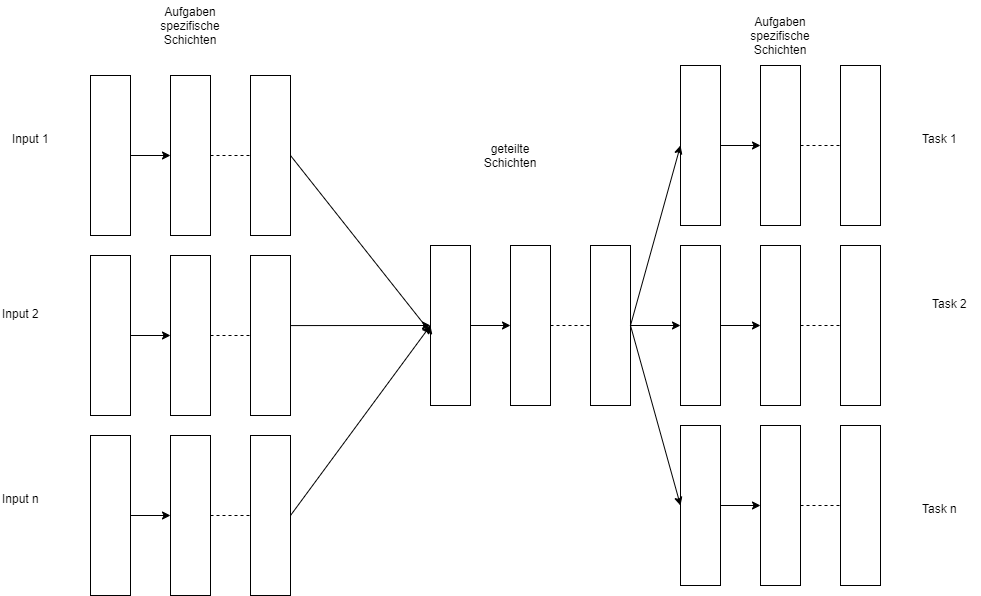
\includegraphics[width=1\textwidth, center]{bilder/Grundlagen/MTL/MTL_MIMO.png}
				\caption[MTL-MIMO]{Multi-Input Multi-Output}
				\label{img:MTL-MIMO}	
			\end{subfigure}
			\caption{Multi-Task-Lernen: Ausprägungen}
			\label{img:MultiTaskLernen}
		\end{figure}
		Abbildung \ref{img:MultiTaskLernen} zeigt die verschiedenen Ausprägungen künstlicher neuronaler Netze, die auf \ac{mtl} beruhen.
		
		Induktives Transferlernen und \ac{mtl} wird darin unterschieden, dass beim induktiven Transferlernen angenommen wird, dass es eine Hauptaufgabe und eine Nebenaufgabe gibt. Die Nebenaufgabe bietet zusätzliche Informationen, um die Hauptaufgabe zu verbessern, bzw. zu generalisieren. Im \ac{mtl} gibt es keine solche Unterscheidung, die Aufgaben werden gleichberechtigt betrachtet. Induktives Transfer-Lernen kann deshalb als Sonderform des \ac{mtl} gesehen werden. \cite{Thung.2018} \cite{Pan.2010}
		
		\todo{related work MT-Learning}
		

	\section{Automatisiertes maschinelles Lernen}
	\label{sec:AutoML}
	Das \acl{automl} kurz \ac{automl} hat das Ziel alle Aspekte des maschinellen Lernens und der Datenanalyse-Pipeline zu automatisieren. Die vollständige Automatisierung erlaubt es auch Nutzern, ohne oder mit geringen Kenntnissen von ML-Techniken, die Erstellung von ML-Systemen durchzuführen.
	Die vollständige Automatisierung ist ein langfristiges Ziel. Aktuelle Systeme sind halbautomatisch und zielen darauf ab, Personenaufwände bei Bedarf nach und nach durch Rechenvorgänge zu reduzieren. Trotz der steigenden Rechenleistung, können AutoML-Methoden sehr rechenintensiv sein.  \ac{automl} wird in drei Methoden eingeordnet. Das Meta-Learning, \acl{nas} kurz \ac{nas} und \acl{hpo} kurz \ac{hpo}. \cite{Hutter.2019} 
	
	\subsection{\acl{hpo}}
	\label{subsec:HyperparameterOptimierung}	
	Hyperparameter sind alle Parameter, welche vor Beginn des Trainings zur Steuerung des Trainings eingestellt werden können. Eine passende Einstellung dieser Parameter beeinflusst die Leistung eines Modells maßgeblich. In \cite{Kohavi.1995} wurde festgestellt, dass verschiedene Hyperparameterkonfigurationen für verschiedene Datensätze am besten funktionieren. Es ist also notwendig für jede Aufgabe aufs Neue die beste Hyperparameterkonfiguration zu finden.      
	Automatische-\ac{hpo} ist die Technik des automatischen Finden der Hyperparameter, um die Leistung zu optimieren. Dabei hat sie insbesondere drei Ziele: An erster Stelle sollen Personenaufwände bei der Anwendung von maschinellem Lernen reduziert werden, zusätzlich soll es die Leistung von Algorithmen und Modellen des maschinellen Lernens verbessern. Des Weiteren sollen so in der Wissenschaft die Reproduzierbarkeit und Fairness von Studien verbessert werden, da Automatische-\ac{hpo} einfacher reduzierbar ist, als manuelle-\ac{hpo}. In Kapitel \ref{subsec:Optimierungstechniken} werden einige gängige Optimierungstechniken der automatischen-\ac{hpo} erläutert.  \cite{Feurer.2019}		
	
	
	\subsection{Meta-Learning}
	\label{subsec:MetaLearning}
	Unter \cite{JoaquinVanschoren.2018} ist eine Übersicht über das Meta-Learning zu finden. In dieser Arbeit wird das Thema nur vollständigkeitshalber aufgelistet. Meta-Learning umfasst jede Art von Lernen, welches auf frühere Erfahrungen zurückgreift. Dabei können umso mehr Arten von Metadaten genutzt werden je ähnlicher die Aufgaben sind. Metadaten sind dabei alle Daten, die frühere Lernaufgaben beschreiben. Dies können z.B Algorithmuskonfigurationen, Hyperparameter, Netzarchitekturen, Modellbewertungen und vieles mehr sein.
	
	\subsection{Neural Architecture Search}
	\label{subsec:NeuralArchitectureSearch}
	Im Deep Learning hängt die Leistung eines Modells maßgeblich von der genutzten Architektur ab. Das manuelle Suchen von Architekturen ist zeitaufwendig und fehleranfällig. Die Neural Architecture Search befasst sich damit, wie Architekturen automatisch gefunden werden können. In dieser Arbeit wurde nicht auf die Technik der Neural Architecture Search zurückgegriffen und das Thema ist nur vollständigkeitshalber aufgeführt. Unter \cite{Elsken.2019} kann eine Übersicht über die Neural Architecture Search gefunden werden. 	

	\subsection{Optimierungstechniken}
	\label{subsec:Optimierungstechniken}
	In diesem Unterkapitel werden gängige Optimierungsmethoden des \ac{automl} dargestellt. Die Auflistung ist nicht vollständig, deckt aber die im praktischen Teil der Arbeit zur Verfügung stehenden Methoden ab.  
	
	\subsubsection{Rastersuche}
	Die Rastersuche ist eine modellunabhängige Optimierunsstrategie. Es werden Parameterkombinationen definiert und anschließend Modelle, ausgehend von den Kombinationen, erstellt und evaluiert. Diese Technik hat einige Schwächen, so müssen Parameterkombinationen definiert werden, jedes Modell muss trainiert werden und falls die optimale Konfiguration nicht enthalten ist, wird sie nie gefunden. \cite{Michelucci.2018}
	
	\subsubsection{Zufallssuche}
	Die Zufallssuche ähnelt der Rastersuche. Sie unterscheidet sich dahingehend, dass die Parameterkombinationen nicht mehr definiert werden müssen. Es werden zufällige Stichprobenkonfigurationen aus dem (definierten) Parameterraum gezogen und evaluiert. 
	In \cite{BergstraJamesandYoshuaBengio..2012} wurde gezeigt, dass insbesondere bei unterschiedlicher Wichtigkeit der Hyperparameter, bessere Ergebnisse erzielt werden. 

	\subsubsection{Bayesian optimization}
	Bayesian optimization ist ein Ansatz der zur Optimierung von Zielfunktionen dient, die eine lange Zeit (Minuten oder Stunden) zur Auswertung benötigen. Im Gegensatz zur Rastersuche oder Zufallssuche ist der Ansatz modellabhängig. Der Ansatz ist iterativ und baut auf zwei Komponenten auf. Ein probabilistisches Ersatzmodell und eine Erfassungsfunktion, die zur Bewertung, welcher Punkt als nächstes bewertet werden soll, herangezogen wird. Das Ersatzmodell wird in jeder Iteration an alle Beobachtungen angepasst. Im Gegensatz zur Blackboxfunktion, ist die Auswertung der Erfassungsfunktion billig und kann somit zur Optimierung herangezogen werden.
	\cite{Frazier.2018}
			
	\subsubsection{Hyperband}	
	Hyperband \cite{Li.2017} erweitert \acl{sh} \cite{Jamieson.2015}. \acl{sh} kurz \ac{sh} weist einer Reihe von Hyperparameter-Konfigurationen eine einheitliche Menge an Ressourcen zu, berechnet die Leistung von allen Konfigurationen und entfernt die schlechtere Hälfte. Die Konfigurationen werden dabei zufällig gezogen. Das Ganze wird wiederholt, bis eine Konfiguration übrig bleibt. In jedem Durchlauf wird der übriggebliebenen Hälfte exponentiell mehr Ressourcen zugewiesen. \ac{sh} benötigt als Eingangsparameter die Ressourcen und die Anzahl an Konfigurationen. Dabei ist es schwierig, zu entscheiden, ob wenige Konfigurationen mit mehr Ressourcen oder viele Konfigurationen mit weniger Ressourcen durchgeführt werden sollen.
	Hyberband erweitert \ac{sh}, um dieses Problem zu adressieren. Hyperband führt eine Rastersuche für die beiden Parameter durch. Es werden also mehrere \ac{sh}-Durchläufe mit diversen Konfigurationen durchgeführt. Die Anzahl an Konfigurationen wird dabei immer weiter reduziert. Abgeschlossen wird eine Ausführung mit einer Zufallssuche.
	
	\subsubsection{BOHB}
	BOHB \cite{StefanFalkner.2018} ist ein Ansatz, der Bayesian optimization und Hyperband kombiniert. Dabei wird Bayesian optimization zur Auswahl von Konfigurationen herangezogen und Hyperband bestimmt wieviele Konfigurationen, mit welchem Budget ausgeführt werden sollen. Anschließend werden die Konfigurationen mittels Successive Halving ausgeführt. Unter https://github.com/automl/HpBandSter kann eine Implementierung des Werkzeuges gefunden werden. Diese Framework wurde für den praktischen Teil der Arbeit genutzt.
			
	\section{Bibliotheken und Werkzeuge}
	\label{sec:BibliothekenundWerkzeuge}
	Für den praktischen Teil der Abschlussarbeit wurde insbesondere Cnvrg \cite{cnvrg.io.2020} genutzt. Cnvrg.io ist eine 'full-stack' Data Science Platform, welche Werkzeuge für die Erstellung, Verwaltung, Bereitstellung und Automatisierung von maschinellem Lernen bereitstellt. Cnvrg erlaubt es Arbeitsbereiche mittels Container zu erstellen. Die Container können dabei auf Maschinen in Azure \cite{Micorsoft.2020} zugreifen. Für die Experimente wurde ein vorgefertigter Container mit einer tesla-k80 \cite{Nvidia.2020}, fünf CPUs und 49 GB Arbeitsspeicher genutzt. 

	Für die Entwicklung wurden Python \cite{PythonSoftwareFoundation.2020}, Jupyter Notebooks \cite{ProjectJupyter.} und das Framework Tensorflow \cite{MartinAbadi.2015}  genutzt. Die wichtigsten Bibliotheken für die Arbeit sind Keras \cite{Chollet.2015} , Numpy \cite{Oliphant.2006} , Matplotlib \cite{Hunter.2007} , scikit-learn \cite{Pedregosa.2011} , ConfigSpace \cite{Lindauer.2019} , Bayesian Optimization and Hyperband \cite{StefanFalkner.2018}. 
	
	Für die Visualisierung von Bildeinbettungen wurde die Software 'PSIORI Visualizer' erweitert und eingesetzt. Die Software erlaubt es dreidimensionale Daten darzustellen. Dabei können Filter eingesetzt sowie Blickwinkel geändert werden, Daten können mit zusätzlichen Informationen versehen werden und Zoomen ist möglich. Als zusätzliche Information können z.B. ein Originalbild und seine Rekonstruktion oder die Information, ob eine Vorhersage korrekt oder falsch war hinterlegt werden.
	
	Kern der erstellten Softwaremodule ist das Framework  Psipy \cite{PSIORIGmbH.2019}. Psipy ist ein Python-Framework für maschinelles Lernen, welches von PSIORI selbst entwickelte Werkzeuge zusammenfasst und unter einer einheitlichen API zu Verfügung stellt. Diese API ist an die API des verbreiteten Frameworks scikit-learn angelehnt. Es können Modelle basierend auf scikit-learn  und Tensorflow eingebunden werden. In den nachfolgenden Abschnitten werden die, für die Arbeit, wichtigsten bestehenden Module des Frameworks vorgestellt.
	
	 \paragraph{saveable.py} Das Modul saveable ist eine flexible Basisklasse, die Kernfunktionalität zum Speichern und Laden von Python-Objekten bietet. Es können Modelle, welche diverse Bibliotheken nutzen, auf eine einheitliche Art und Weise gespeichert werden. Um die Klasse Saveable nutzen zu können, müssen erbende Klassen ihre Konstruktorargumente an die Basisklasse übergeben. Zusätzlich ist es notwendig eine Erweiterung beim Speichern und Laden zu implementieren. Beim Speichern ist es notwendig eine Erweiterung, um alle (meist ein) Module und weitere Argumente zu implementieren. Beim Laden müssen die gespeicherten Module und Argumente geladen werden. In Listing \ref{lst:SaveTensorflow} ist die Erweiterung zum Speichern eines Tensorflow-Models abgebildet. 
	\begin{lstlisting}[language=python,caption=Erweiterung zum Speichern eines Tensorflow Models, label=lst:SaveTensorflow]
		...
		zip_file.add("model.h5", self.model)
		...
	\end{lstlisting}

	\paragraph{autoencoder.py} Das Modul autoencoder enthält die drei Klassen StackedAutoencoder, FullyConnectedAutoencoder und ConvolutionalAutoencoder. Der StackedAutoencoder wird als Basisklasse für die anderen beiden Klassen genutzt. Im Konstruktor werden Methoden aufgerufen, welche in den abgeleiteten Klassen ausprogrammiert sind. Dabei wird ein Keras-Modell für einen Encoder und Decoder entsprechend von Parametern erstellt. Als weitere wichtige Methoden gibt es die Methode $pretrain(..)$ und $fit(..)$. Mittels $pretrain(..)$ werden die Schichten eines symmetrischen Autoencoder von außen nach innen wie, in \cite{Bengio.2007} beschrieben vortrainiert. Die Zuordnung der Schichten erfolgt in den abgeleiteten Klassen.
	In der $fit(..)$-Methode wird nach einigen Prüfungen die Methode f$fit(..)$ \cite{Chollet.2015} des Kerasmodels aufgerufen. In Abbildung \ref{img:KlassendiagrammConvolutionalAutoencoder} ist das Klassendiagramm mit den öffentlichen Methoden des ConvolutionalAutoencoder dargestellt. 
	\begin{figure}[h]
		\centering
		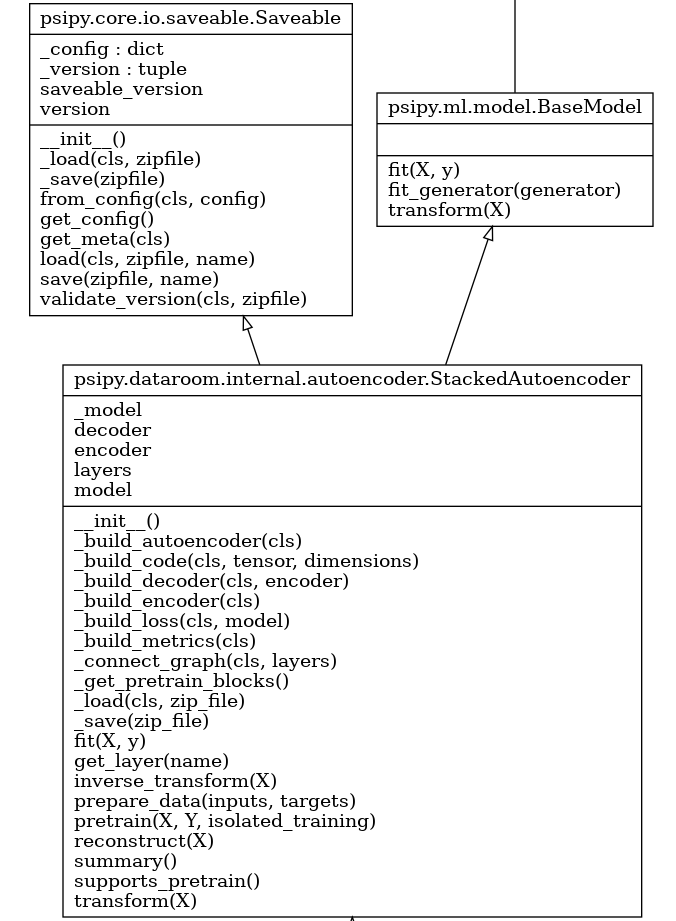
\includegraphics[width=0.6\textwidth, center]{bilder/Klassendiagramme/klassendiagramm_public_cae2.png}
		\caption[Klassendiagramm ConvolutionalAutoencoder]{Klassendiagramm ConvolutionalAutoencoder}
		\label{img:KlassendiagrammConvolutionalAutoencoder}
	\end{figure}  
	
	\paragraph{hyperparameter\_mixin.py}  Hyperparameter\_mixin wird zum standardisierten Verwalten von Hyperparametern für AutoML-Klassen genutzt. Auf die Hyperparameter kann anschließend einheitlich zugegriffen werden. Abbildung \ref{img:KlassendiagrammHyperparametermixin} zeigt das zugehörige UML-Klassendiagramm mit den Methoden zum Hinzufügen, Löschen und Laden der Hyperparameter. Da die Methoden öffentlich sind, können über jede erbende Klasse die Hyperparameter eigenständig verwaltet werden.	
	\begin{figure}[h]
		\centering
		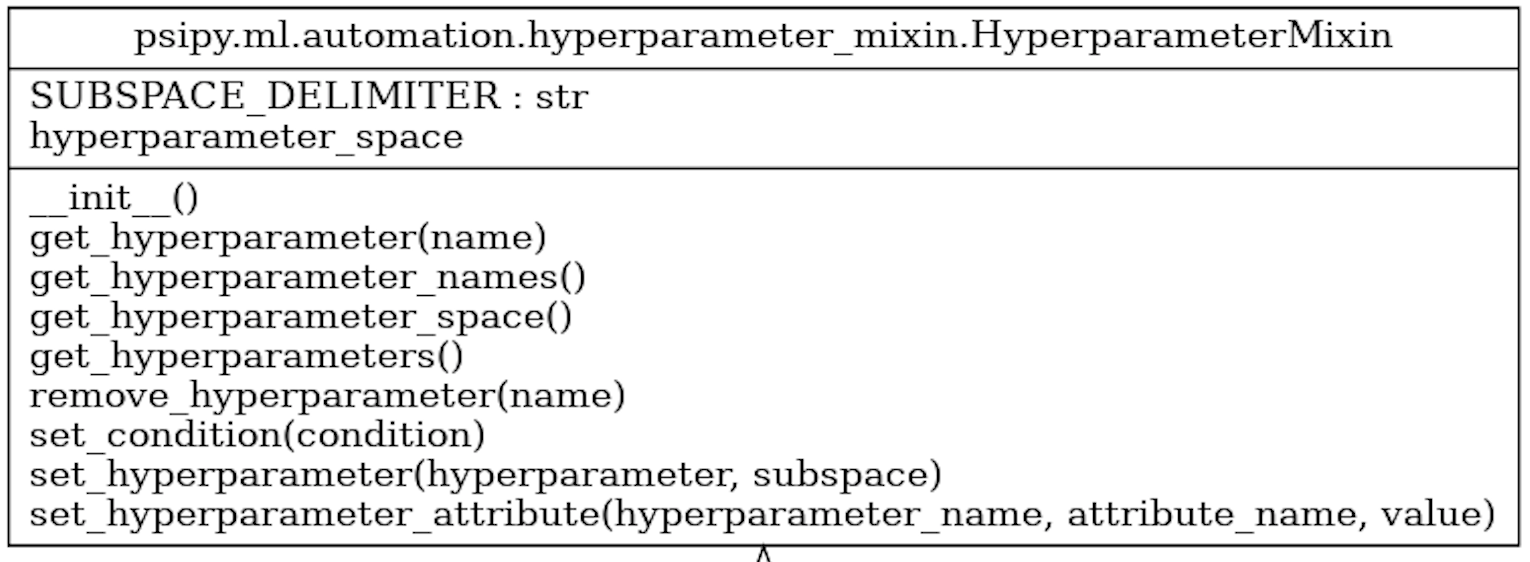
\includegraphics[width=0.5\textwidth, center]{bilder/Klassendiagramme/Hyperparametermixin.png}
		\caption[Klassendiagramm Hyperparametermixin]{Klassendiagramm Hyperparametermixin}
		\label{img:KlassendiagrammHyperparametermixin}
	\end{figure}  
	
	\section{Einordnung und bestehende Systeme}
	\label{sec:BestehendesSystem}
	Die Bilddaten und Aufgabenstellungen der neuronalen Netzwerke sind in die Problemstellungen des Autocrane-Projekts von PSIORI einzuordnen. Es sind echte Datensätze und echte Problemstellungen, wobei die gezeigten Aufgabenstellungen und Modelle nicht zwingend in dem Autocrane-Projekt zum Einsatz kommen. Das Autocrane-Projekt ist ein (laufendes) Projekt, welches das Ziel hat, einen feststehenden Rundlaufkran vollautomatischen zu steuern. In Abbildung \ref{img:CircularCrane} ist ein Rundlaufkran abgebildet. Diese Art von Kran werden in holzverarbeitenden Anlagen zum Befüllen von Fülltrichtern oder Förderbändern eingesetzt. Der Kran kann sich um 360 Grad drehen. Der Greifer kann nach oben, unten und mittels eines Schlittens entlang eines Auslegers bewegt werden. Um die Bilder aufnehmen zu können, wurde an der Kabine am Hauptstandfuß eine Kamera angebracht. Die Kamera ist auf das Ende des Auslegers und den Bereich darunter ausgerichtet. Die Kamera bewegt sich mit dem Rundlaufkra, wodurch der Greifer immer im Bild ist. Für das Autocarne-Projekt sind insbesondere drei Anwendungsfälle interessant. Die Baumstämme werden mittels LKW angeliefert und müssen nach vorgegebenen Regeln (z. B. Ausrichtung, freier Lagerplatz) als Holzstapel gelagert werden. Der Fülltrichter muss mit Holz aus den Holzstapeln befüllt werden. Der Fülltrichter muss mit Holz aus einem LKW befüllt werden. Es ergeben sich Aufgabenstellungen wie Greifer-Erkennung, Baumstamm-Erkennung, LKW-Erkennung, Strategien für das Entladen und Aufbewahren der Baumstämme und vieles mehr. Im Normalbetrieb werden täglich 140-200 LKW entladen. Die Ladung ist 9 - 18 Meter lang und 34 - 40 Tonnen schwer. \cite{PSIORIGmbH.2020}
	\begin{figure}[h]
		\centering
		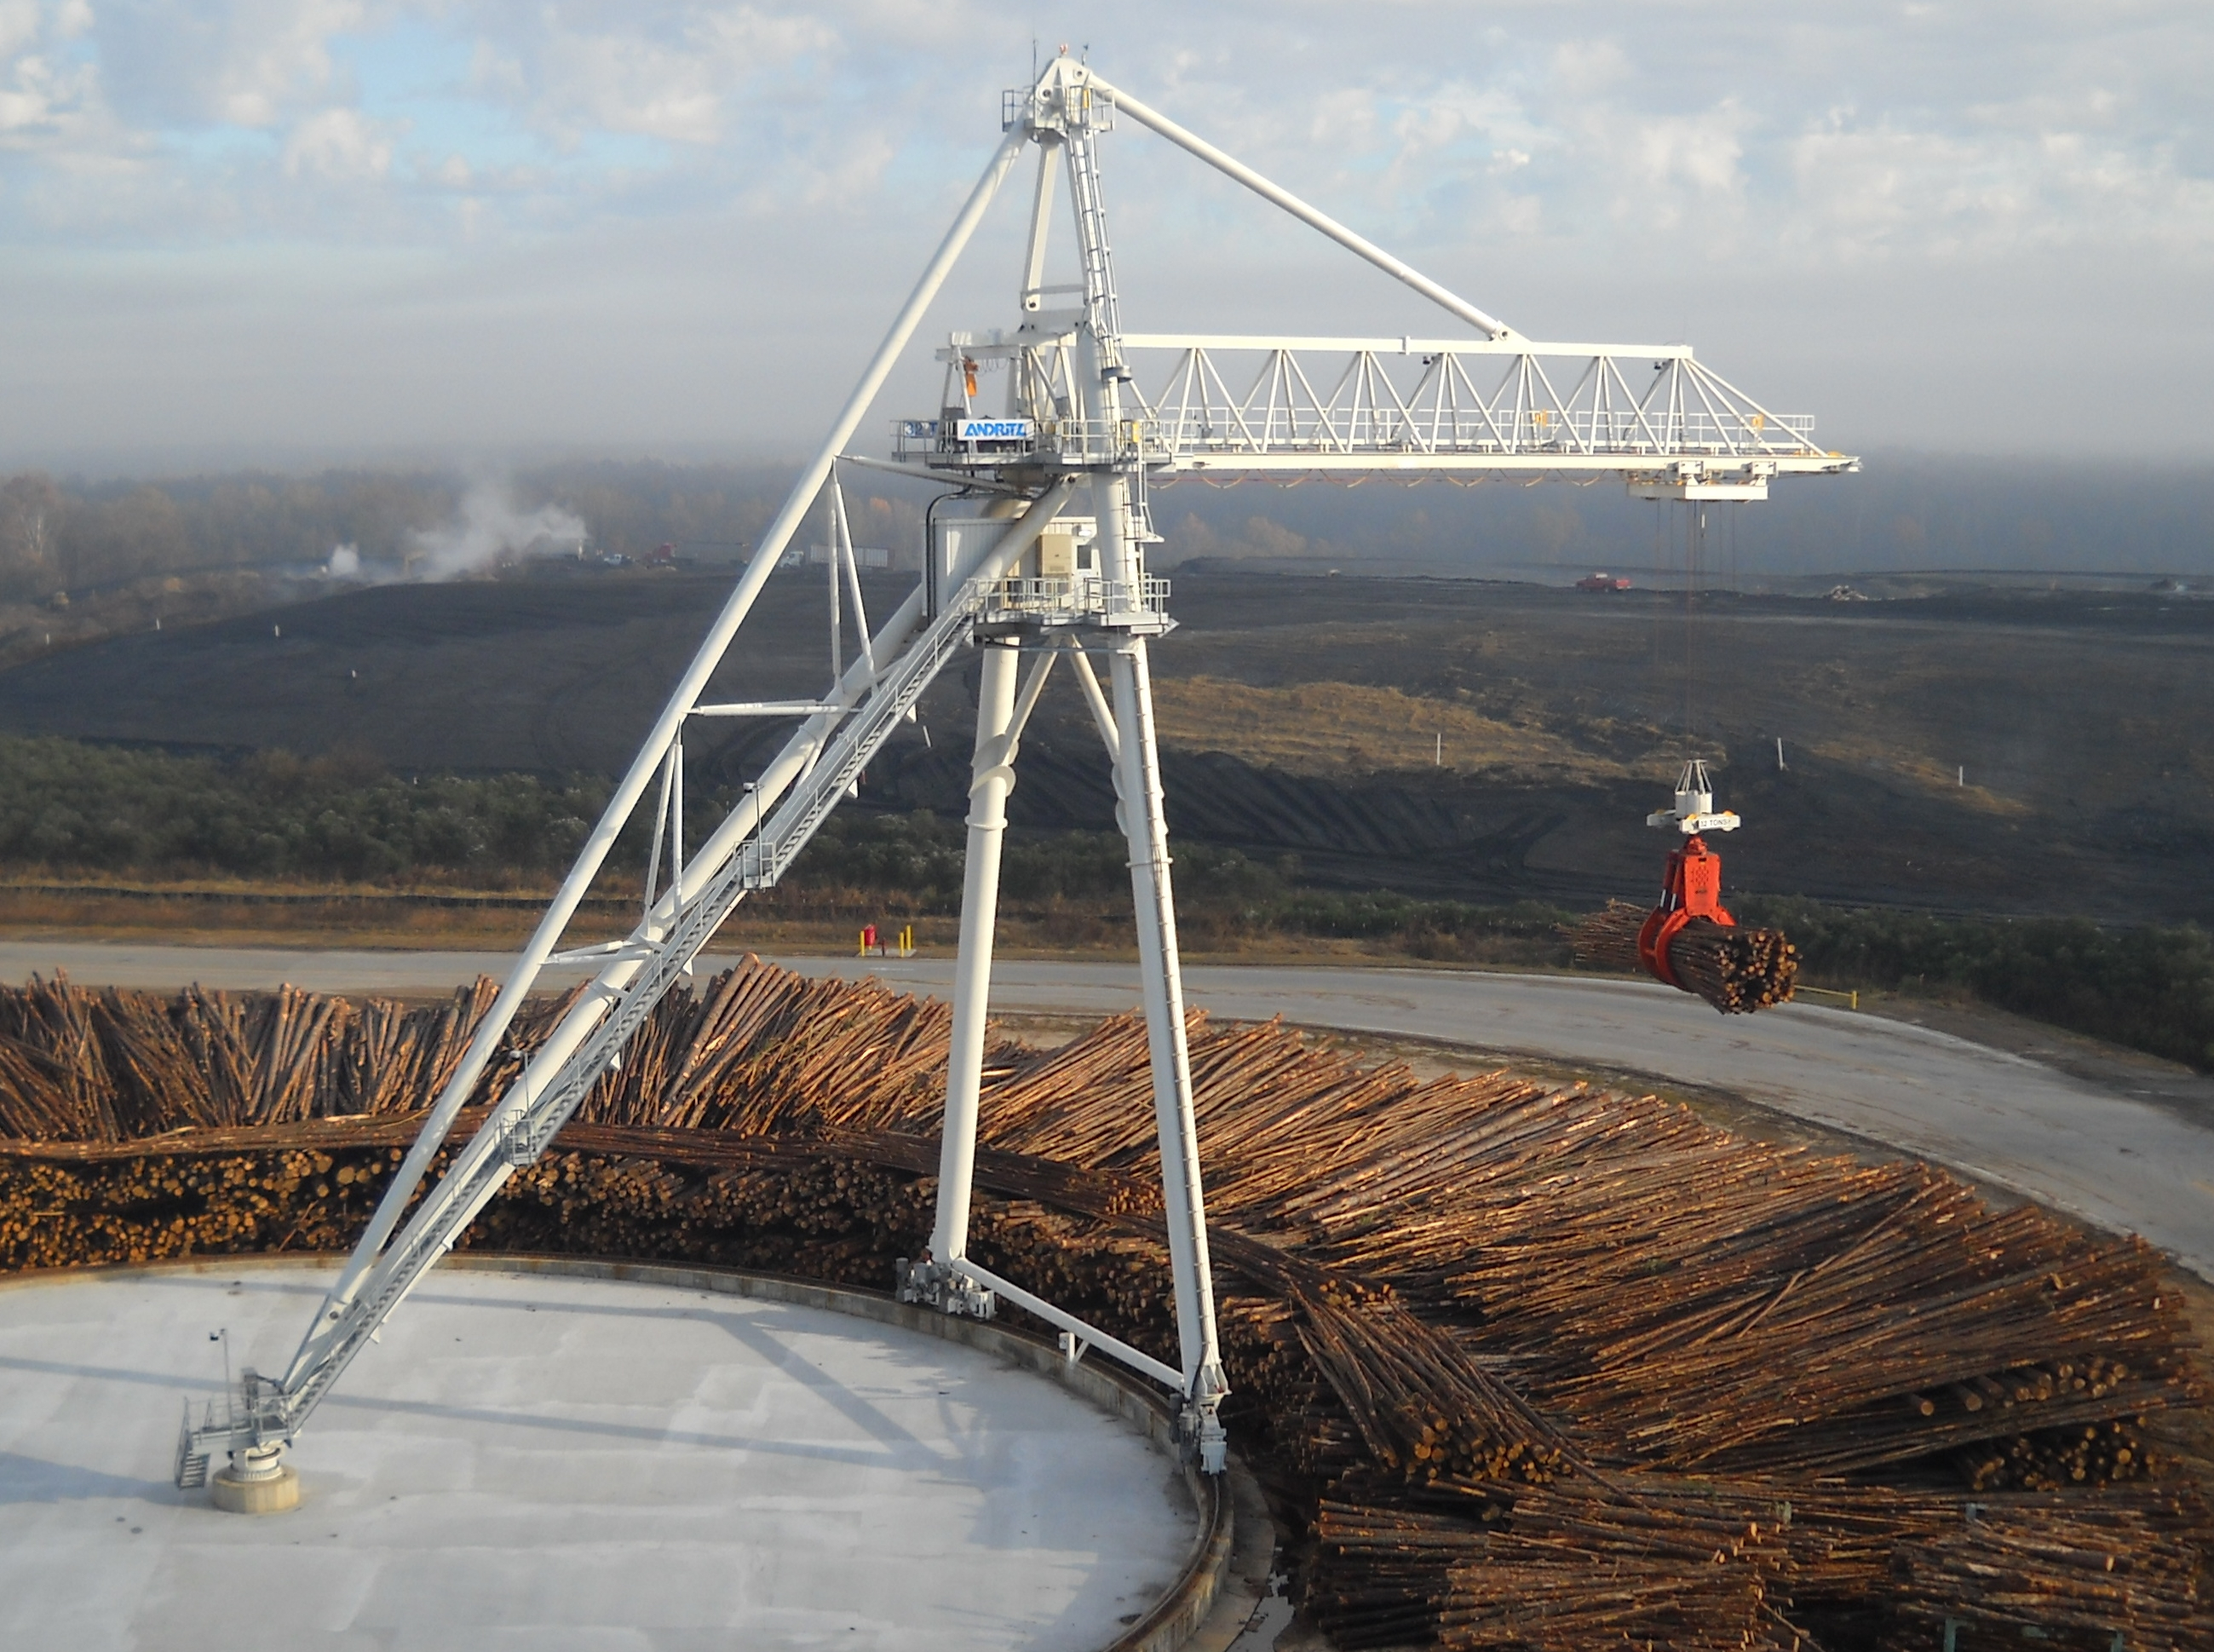
\includegraphics[width=0.5\textwidth, center]{bilder/Grundlagen/Kran_vollstaendig_N1_030.jpg}
		\caption[Rundlaufkran]{Rundlaufkran (Foto: ANDRITZ)}
		\label{img:CircularCrane}
	\end{figure}		

	\paragraph{Greifererkennung} Bei der Aufgabenstellung Greifererkennung muss in einem Bild die Position eines Rahmen um den Greifer gefunden werden. Abbildung \ref{img:Grapple} zeigt ein Bild eines Rahmens um den Greifer. Es handelt sich um eine klassische Objekterkennungs-Aufgabe.
	\begin{figure}[h]
		\centering
		\begin{subfigure}[c]{0.49\textwidth}			
			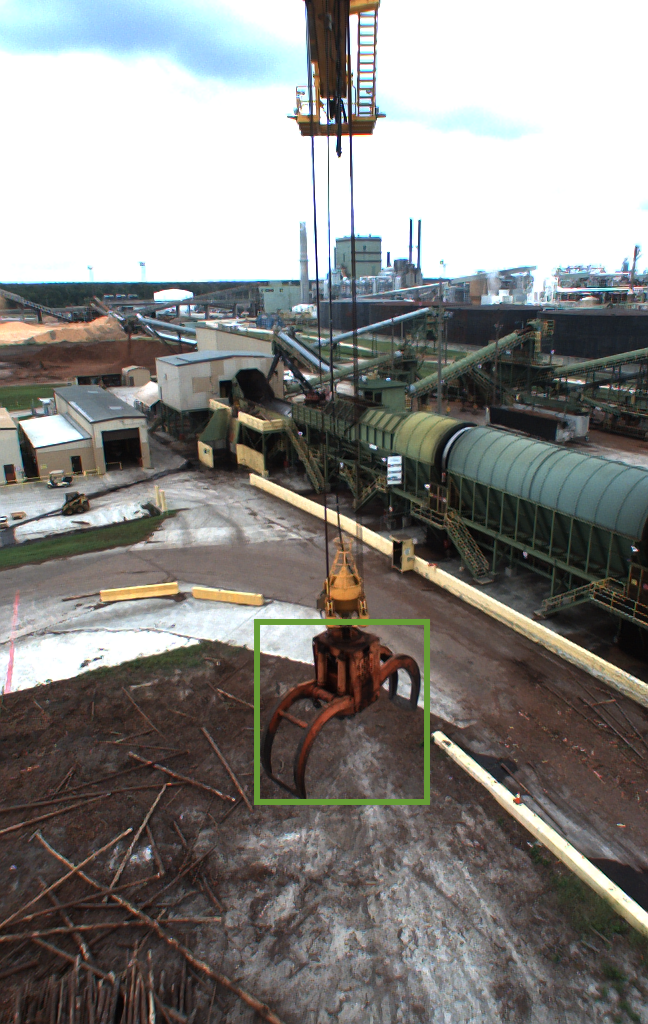
\includegraphics[width=1\textwidth, center]{bilder/Grundlagen/Grapple_8.png}
			\caption[Bsp. Bild: Greifer mit Rahmen]{Greifer mit Rahmen}
			\label{img:Grapple}	
		\end{subfigure}
		\begin{subfigure}[c]{0.49\textwidth}			
			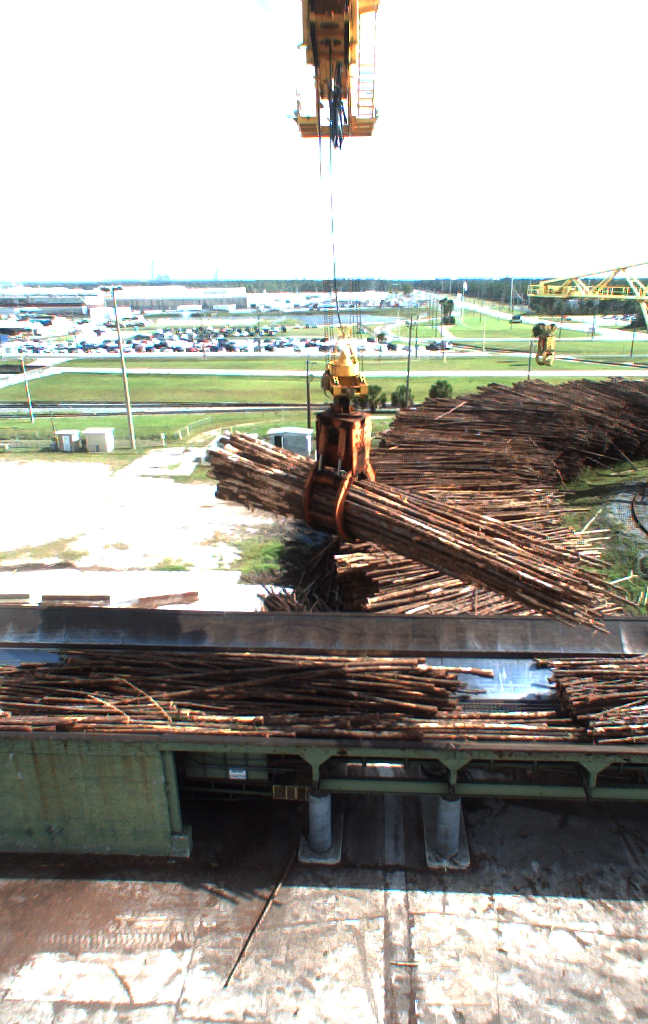
\includegraphics[width=1\textwidth, center]{bilder/Grundlagen/Logs_14.png}
			\caption[Bsp. Bild: Greifer mit Baumstämmen]{Greifer mit Baumstämmen}
			\label{img:Logs}	
		\end{subfigure}
		\caption{Greifer}
		\label{img:Greifer}
	\end{figure}	

	PSIORI hat die Aufgabe mittels neuronalem Netzwerk gelöst. Dabei wurde auf die Technik des Single Shot MultiBox Detector (SSD) \cite{Liu.2015} zurückgegriffen. Die Vorhersagegenauigkeit dieses Modells wird als Basislinie und Vergleichswert genutzt. Dabei ist die ausschlaggebende Metrik die  \acl{iou} kurz \ac{iou} mit einem Schwellenwert von 0.8. Es wird also die Fläche der Überschneidung der beiden Rahmen durch die Gesamtfläche der Rahmen geteilt und wenn ein Wert >= 80\% erreicht wird, als korrekt vorhergesagt eingestuft.  Das Modell erreicht einen Wert von $0.86$. In Anhang \ref{appendix:BasislinieGreifer} ist die vollständige Basislinie dargestellt.
	
	\paragraph{Greifer beladen} Die Aufgabe 'Greifer beladen' hat zum Ziel, zu erkennen ob sich Baumstämme im Greifer befinden oder nicht. Es handelt sich um eine Klassifikationsaufgabe. Für diese Aufgabe wurde von PSIORI ein Modell erstellt. Dieses Modell wird wie das Greifererkennungsmodell als Basislinie und Vergleichswert für die durchgeführten Versuche genutzt. Das Modell erreicht auf den Validation-Daten eine Accuracy von 0.9828\%. Im Anhang \ref{appendix:BasislinieBaumstämme} ist die vollständige Basislinie dargestellt. 

	\section{Datenverständnis}
	\label{sec:DataUnderstanding}
	Mittels Kamera an der Kabine können neue unbeschriftete Bilder aufgenommen und bei PSIORI abgelegt werden. Durch den Aufbau des Rundkrans und der Kameraposition, befindet sich der Greifer immer im Bild. Der Hintergrund der Bilder ändert sich stark. Die geografische Lage des Rundkrans schränkt die möglichen Wetterlagen ein. Es fällt kein Schnee und es gibt wenige Regentage. In Abbildung  \ref{img:Bildqualität} sind Ausprägungen der Bildqualität dargestellt. Abgesehen von Bildern in guter Qualität gibt es helle Bilder, dunkle Bilder und Bilder mit Reflexionen. Die Bilder sind 1024 auf 648 Pixel groß und in Farbe. Die einzelnen Pixel können dabei Werte zwischen 0 und 255 annehmen. 
	Entsprechend der beiden Aufgabenstellungen Greifererkennung und 'Greifer beladen' werden Daten mit einer passenden Beschriftung bereitgestellt.
	
	\begin{figure}[h]
		\centering
		\begin{subfigure}[c]{0.24\textwidth}			
			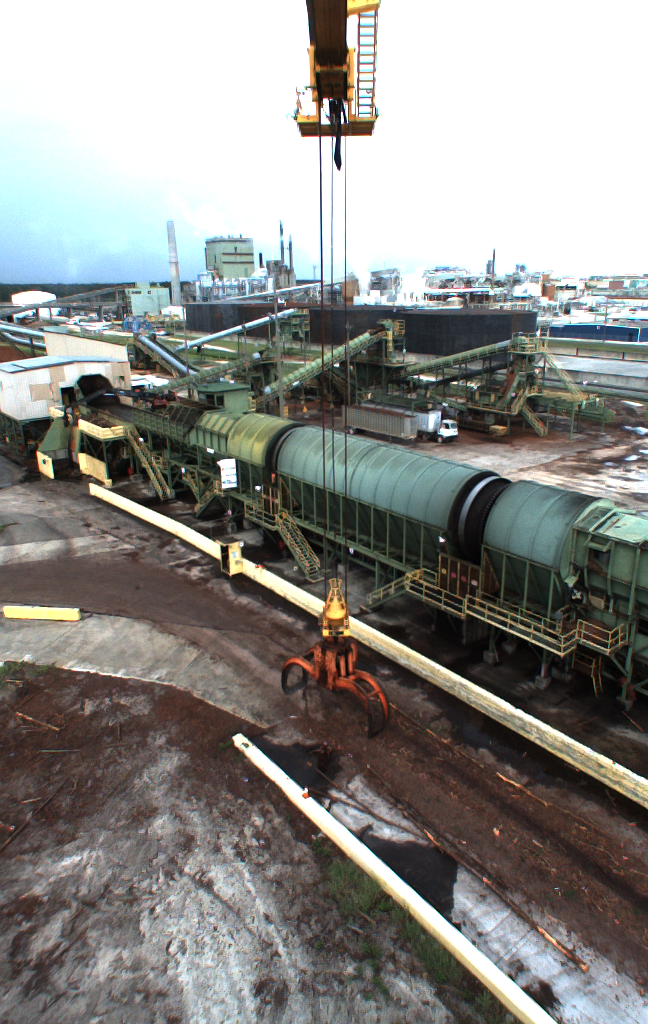
\includegraphics[width=1\textwidth]{bilder/Grundlagen/Daten_Bildqualitaet/gut.png}
			\subcaption{Gut}			
		\end{subfigure}
		\begin{subfigure}[c]{0.24\textwidth}			
			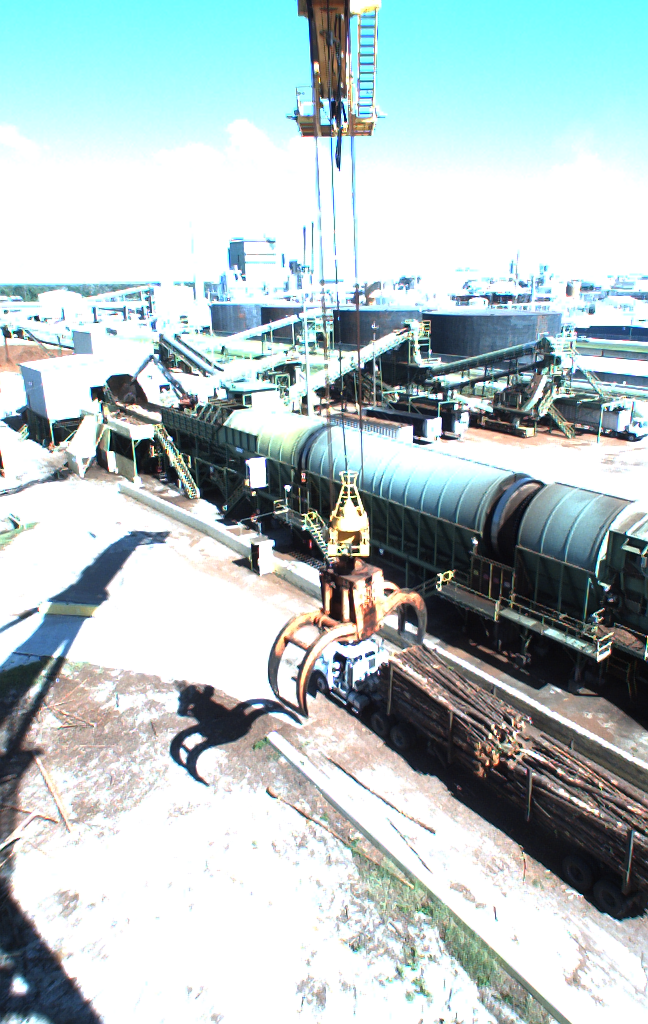
\includegraphics[width=1\textwidth]{bilder/Grundlagen/Daten_Bildqualitaet/hell.png}
			\subcaption{Hell}			
		\end{subfigure}
		\begin{subfigure}[c]{0.24\textwidth}			
			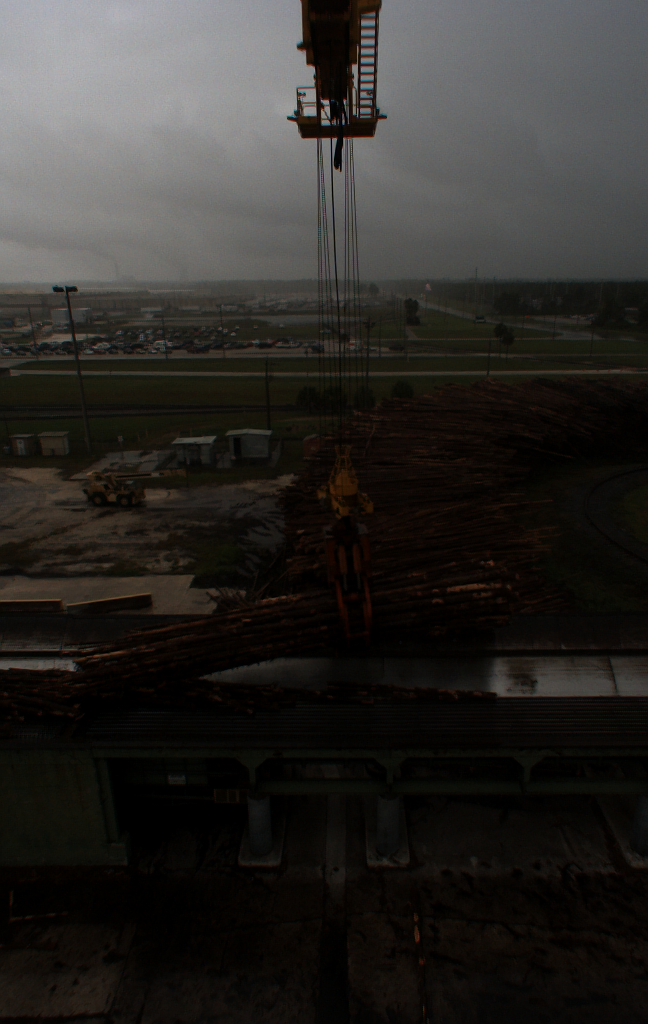
\includegraphics[width=1\textwidth]{bilder/Grundlagen/Daten_Bildqualitaet/dunkel.png}
			\subcaption{Dunkel}			
		\end{subfigure}
		\begin{subfigure}[c]{0.24\textwidth}			
			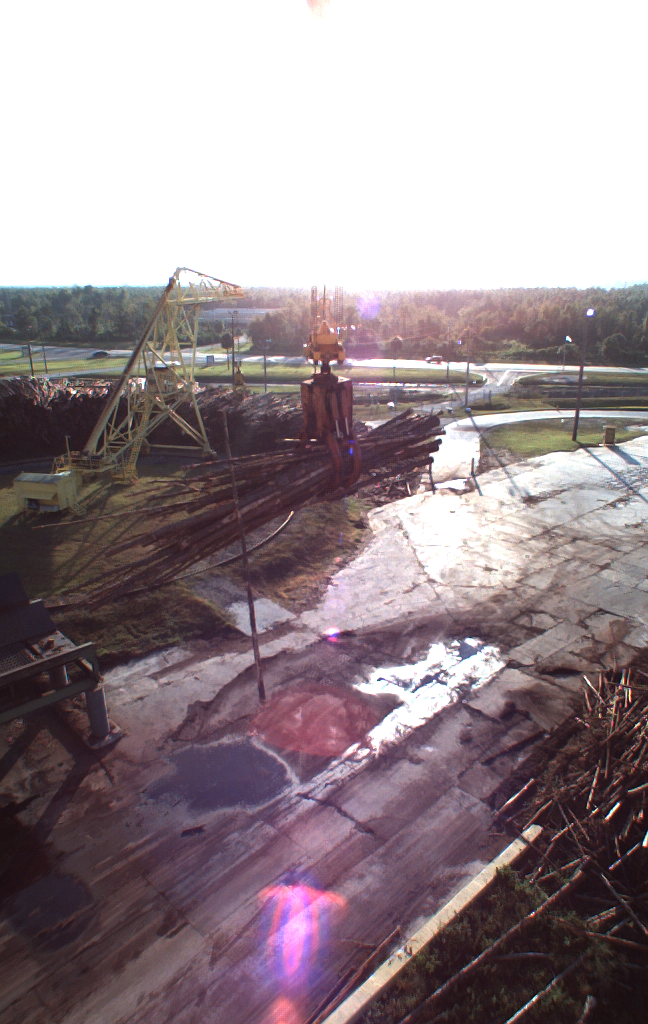
\includegraphics[width=1\textwidth]{bilder/Grundlagen/Daten_Bildqualitaet/Reflexionen.png}
			\subcaption{Reflexionen}			
		\end{subfigure}
		\caption{Bildqualität}
		\label{img:Bildqualität}
	\end{figure}
		
	\paragraph{Greiferdatensatz} Der Greifer Datensatz enthält Bilder, in welchen der Greifer mittels Rahmen markiert ist. Abbildung \ref{img:Grapple} zeigt ein beispielhaftes Bild mit markiertem Greifer. Die Annotationen der Position des Greifers wurde pro Bild in einer XML-Datei abgelegt. Konkret wurde die Position als x, y Koordinaten in der Form ymin, xmin, ymax und xmax abgespeichert. Über die vier Werte lässt sich problemlos ein Rahmen um den Greifer spannen. Der Datensatz besteht aus 4.684 durch Personen annotierten Bildern.
	
	\paragraph{Generierter Greiferdatensatz}  Erfahrungsgemäß lernen Autoencoder Lichtverhältnisse in Bildern relativ gut. Um für erste Versuche den Fokus von den Lichtverhältnissen auf die eigentliche Aufgabenstellung zu setzen wurde ein weiterer Greiferdatensatz erzeugt. Hierfür wurden 8966 Bilder mittels dem Basislinienmodell beschriftet und in 7171 Trainingsdaten und jeweils 896 Test- und Validationsaten aufgeteilt.
	 
	\paragraph{Baumstammdatensatz} Der Baumstammdatensatz enthält Bilder, welche die Annotation, ob sich Baumstämme im Greifer befinden oder nicht, enthält. Die Bilder sind durch zwei Ordner in Bilder mit und Bilder ohne Baumstämme aufgeteilt. Abbildung \ref{img:Logs} zeigt ein Bild, in welchem der Greifer Baumstämme greift. In Abbildung \ref{img:Grapple} befinden sich keine Baumstämme im Greifer.  
			
	\section{Datenvorbereitung}
	\label{sec:DataPreparation}
	In Vorbereitung auf die Modellierungsphase wurde ein finaler Datensatz erstellt und Werkzeuge zum Laden und Vorbereiten der Daten implementiert.
	\paragraph{Erste Iteration} Als Erstes wurden die Daten mittels Skripten in Training, Test und Validation Daten aufgeteilt. Anschließend wurden die Daten auf der Cnvrg-Plattform in einen versionierbaren Datenspeicher geladen. In Tabelle \ref{table:DatenaufteilungTrainTestValidation} ist die finale Datenaufteilung zu sehen. Die Greifer Daten sind in 70\% Trainingsdaten und jeweils 15\% Test und Validierungsdaten aufgeteilt. Die Baumstammdaten sind in 80\% Trainingsdaten, 10\% Testdaten und 10\% Validierungsdaten getrennt worden. Die Trainingsdaten werden zum Trainieren der Modelle genutzt, die Testdaten zum Überprüfen der Modelle und die Validierungsdaten werden am Ende der Experimente für die finale Überprüfung der Ergebnisse eingesetzt.
	\begin{table}[ht]
		\centering
		\begin{tabularx}{\textwidth}{lllll}
			& \textbf{Train} & \textbf{Test}  & \textbf{Validation} & \textbf{Summe} 	 \\
			\textbf{Greifer} 				 & 	3.279			& 703	 & 704				   & 4.686 	\\
			\textbf{Baumstämme j/n}	 	  &  9.749	   & 1.221 	& 1.225	& 12.195\\		
		\end{tabularx}
		\caption{Datenaufteilung - Train Test Validation}
		\label{table:DatenaufteilungTrainTestValidation}
	\end{table}
	
	Für das Laden der Daten wurde ein Modul 'data\_loader.py' erstellt. Dieses Modul enthält die drei Klassen DataLoader, GrappleDataLoader, LogsDataLoader. DataLoader ist eine abstrakte Klasse, welche Methoden zum Laden der Train-, Test- und Validationdaten definiert. Sie liefern entsprechend eines Parameters, bis zur maximalen Anzahl an Bildern, Bilder als Numparray zurück. Die Klassen GrappleDataLoader und LogsDataLoader implementieren für den jeweiligen Datensatz die konkreten Methoden zum Laden der Daten.
	
	Mittels des Moduls 'data\_preparation.py' und der Klasse Preprocessing werden die Bilder auf die passende Größe verkleinert oder vergrößert und auf den Wertebereich zwischen 0 und 1 normalisiert.
	
	\paragraph{Zweite Iteration} 
	In der zweiten Iteration wurde ein neues Modul namens data\_generator\_provider.py erstellt. Da Bilder als Numpyarray direkt in den Speicher geladen werden, können nicht beliebig viele Bilder genutzt werden. Dieses Problem wird von den Keras ImageDataGeneratoren \cite{Chollet.2015} adressiert. Sie erlauben es Bilder stapelweise bereitzustellen. Zusätzlich können die Imagedatageneratoren die Bilder direkt in der benötigten Größe bereitgestellt werden. Das Modul implementiert jeweils für den Baumstamm Datensatz und den Greiferdatensatz eine Klasse zum Bereitstellen von Imagedatageneratoren.
	
	Da die Modelle \ac{simo}-Modelle sind, erfolgt zusätzlich noch eine Aufbereitung der Bereitstellung der Daten. Standardmäßig stellen die Generatoren Stapel mit Einträgen der Form $X ,Y$  bereit. Wobei X die Eingangsdaten sind und Y die Zielgröße definiert. Zum Beispiel kann X ein Bild sein und Y die zugehörige Klasse. Die Multi-Task-Module benötigen Generatoren, die Einträge der Stapel der Form $X, [X, Y]$ erzeugen. Die Zielgröße hat sich zu einer Liste mit zwei Größen verändert. Die erste Zielgröße entspricht den Eingangsdaten, sie werden für den Decoder-Ausgang genutzt. Die zweite Zielgröße wird für den zweiten Ausgang genutzt. Sie entspricht der Zielgröße eines normalen ImageDataGeneratoren. Das Ganze wird mit Hilfe der Klasse tensorflow.keras.utils.Sequence erreicht. Ihr wird im Konstruktor ein Imagedatagenerator übergeben. Bei der Bereitstellung eines Elementes wird der Rückgabewert des Generators angepasst. Die entscheidenden Codezeilen sind in Listing \ref{lst:AufbereritungGeneratorergebnis} dargestellt. 
	\begin{lstlisting}[language=python,caption=Aufbereitung Generatorergebnis in Python, label=lst:AufbereritungGeneratorergebnis]
		res = self.generator.next()
		return res[0], [res[0], res[1]]
	\end{lstlisting}
	
	Für das Vortrainieren werden Generatoren bereitgestellt, welche Stapel mit Einträgen der Form $X ,X$ erzeugen. Hierbei wird auf Standardfunktionalität der Klasse Imagedatagenerator zurückgegriffen.
	
	Die Imagedatageneratoren bieten Standardfunktionalität zur Bildverstärkung. Alle Generatoren normalisieren die Werte der Bilder zwischen 0 und 1. Die Generatoren für die Trainingsdaten führen noch zufällige Veränderungen der Helligkeit und Kanalverschiebungen durch. Bei den Baumstamm Daten werden die Bilder zusätzlich horizontal umgedreht. 


 


 
